\section{Auswertung}
\label{sec:Auswertung}
\subsection{Vertikalkomponente des Erdmagnetfeldes}
Zu Beginn der Messung wird mit Hilfe einer Vertikalfeld-Spule
die lokale vertikal Komponente des Erdmagnetfeldes kompensiert, damit
 die der zusehende Peak
wie in der Justage beschrieben möglichst schmal wird. Folglich
gilt
\begin{align*}
B_{Erde_z}=B_{vertikal}.
\end{align*}
Das Magnetfeld der Vertikalfeld-Spule lässt sich über die Gleichung
\eqref{eqn:helm},die Magnetischeflussdichte für eine Helmholzspule mit dem Radius $R$,
Anzahl der Windungen $N$, der Magnetischen Feldkonstante $\mu_0$ und dem durchfließenden Strom $I$
\begin{align}
% B=const.mu_0*(8*I*N/(np.sqrt(125)*R))
B=\mu_0 \cdot \frac{8 I N}{\sqrt{125} R}, \label{eqn:helm}
\end{align}
berechen. Bei der Vertikalen-Spule besitzt einen Radius von $R=11,735\,\si{\centi\meter} $
und eine Windungszahl von $N=11$.
Bei einem Strom von
\begin{align*}
  I_{vertikal}=0.22 \,\si{\ampere}
\end{align*}
wird die Peakbreite minimal. Somit folgt aus \eqref{eqn:helm}
eine  vertikal Komponente von
\begin{align*}
  B_{vertikal}=33.7\,\si{\micro\tesla}.
\end{align*}



\subsection{Landesche $g_F$ -Faktoren und horizontal Komponente der Erdmagnetfeldes}
In der Tabelle \ref{tab:messwerte} sind jeweils
für  unterschiedliche Frequenzen der RF-Spule
die eingestellten Ströme $I$ für die "Sweep"- und Horizontal-Spule
und die daraus
berechneten gesamt B-Feldstärken,
bei denen es zu Resonanzen kommt, aufgelistet.
Die gesamt B-Feldstärke resultiert dabei aus
der Summe der B-Feldstärken der
einzelnen Spulen, die sich mit Hilfe der Formel \eqref{eqn:helm}
berechnen lassen.
Die "Sweep"-Spule besitzt einen Radius  $R=16.39\si{\centi\meter}$
und einer Windungszahl $N=11$, bei der Horizontale-Spule ist $R=15,79\,\si{\centi\meter}$
 und $N=154$ .

\begin{table}
\centering
\caption{Messwerte für die Position der zwei Peaks bei unterschiedlichen Frequenzen.}
\label{tab:messwerte}
\begin{tabular}{c| c c c | c c c }
\toprule
Frequenz & \multicolumn{3}{c}{Erster Peak} & \multicolumn{3}{c}{Zweiter Peak} \\
$\nu \, \si{\mega\hertz}$  & $I_{Sweep} \, \si{\per\ampere}$ &   $I_{hori} \, \si{\per\ampere}$ &  $B_{ges} \, \si{\per\micro\tesla}$ & $I_{Sweep} \, \si{\per\ampere}$
&   $I_{hori} \, \si{\per\ampere} $ & $ B_{ges} \si{\per\micro\tesla}$\\
\midrule
0,1 & 0,570 &  0       & 34,40  & 0,690 & 0      &   41,64 \\
0,2 & 0,613 &  0,015   & 50,15  & 0,845 & 0,015  &   64,15 \\
0,3 & 0,198 &  0,060   & 64,57  & 0,555 & 0,060  &   86,11 \\
0,4 & 0,220 &  0,075   & 79,05  & 0,660 & 0,075  &  105,60 \\
0,5 & 0,245 &  0,090   & 93,71  & 0,836 & 0,075  &  116,22 \\
0,6 & 0,045 &  0,120   & 107,95 & 0,760 & 0,120  &  151,10 \\
0,7 & 0,034 &  0,129   & 115,18 & 0,970 & 0,129  &  171,67 \\
0,8 & 0,016 &  0,153   & 135,14 & 0,955 & 0,153  &  191,80 \\
0,9 & 0,307 &  0,150   & 150,07 & 0,712 & 0,195  &  213,98 \\
1,0 & 0,334 &  0,165   & 164,86 & 0,415 & 0,240  &  235,52 \\
\bottomrule
\end{tabular}
\end{table}

Die Messwerte werden in der Form $B_{ges}$ in Abhängigkeit von der Frequenz $\nu$,
zusehen in der Abbildung \ref{fig:mess}, aufgetragen.

\begin{figure}
  \centering
  \includegraphics[width=0.7\textwidth]{build/plot1_messwerte}
  \caption{Messwerte der Stärke der Magnetfeldes für die Position der Peaks bei unterschiedlichen Frequenzen}
  \label{fig:mess}
\end{figure}

Für die Messwerte der zwei Peaks werden zwei linerare Ausgleichsrechnungen
durchgeführt und es ergeben sich die folgenden Werte für die Steigungen und die y-Achsenabschnitte
\begin{align*}
  m_1&= \SI{1,42(3)e-10}{\tesla\per\hertz}&    &b_1=\SI{2,12(15)e-5}{\tesla}\\
  m_2&= \SI{2,15(5)e-10}{\tesla\per\hertz}&    &b_2=\SI{1,93(28)e-5}{\tesla}.
\end{align*}

Aus der Formel \eqref{eqn:keineahnung} folgt
\begin{align}
m=\frac{4\pi m_e}{e_0 g_F} \label{eqn:m}
\end{align}
und
\begin{align*}
b=B_\mathrm{Erde-hori}.
\end{align*}
Somit folgt für die horizontale Komponente der Erdmagnetfeldes durch Mittelung der
beiden berechnenten y-Achsenabschnitte
\begin{align*}
B_\mathrm{Erde-hori}=\SI{20,2(16)}{\micro\tesla}.
\end{align*}
Ebenfalls folgt aus umstellen der Formel \eqref{eqn:m} nach $g_F$
\begin{align}
  g_F=\frac{4\pi m_e}{e_0 m} \label{eqn:g_f}
\end{align}
Durch einsetzen der Steigungen ergibt sich:
\begin{align*}
  g_{F_1} & =0,502\pm0,09 &  & g_{F_2}=0,332\pm0,007
\end{align*}

\subsection{Kernspin}
Aus dem zuvor berechneten Faktoren $g_F$ von dem zwei Isotopen $\ce{^{87}Rb}$ und $\ce{^{85}Rb}$ kann,
durch umstellen der Gleichung \eqref{eqn:JI}
nach $I$ zu
\begin{align}
  I=J\left( \frac{g_J}{g_F}-1\right) \label{eqn:I}
\end{align}
und einsetzten von der Landé-Faktor $g_J\approx2,0023$ der Kernspin für die
unterschiedlichen Isotope brechnet werden.
Es folgt aus \eqref{eqn:I}
\begin{align*}
  I_1&=1,50\pm0,04&   &I_2=2,52\pm0,06.
\end{align*}
Aus einer Nuklidkarte \cite{verhalt} kann entnommen werden, dass für
$\ce{^{87}Rb}$ $I=\frac{3}{2}$
und  für $\ce{^{85}Rb}$ $I=\frac{5}{2}$ gilt.
Folgich kann dem 1. Isotop $\ce{^{87}Rb}$ und dem  2. Isotop $\ce{^{85}Rb}$
zugewiesen werden.
\subsection{Isotopenverhältnis}
Aus einem Sigwnalbild für $\nu=100\,\si{\kilo\hertz}$
zu sehen in der Abbildung \ref{fig:signal},
kann das Isotopenverhältnis bestimmt werden.

\begin{figure}
  \centering
  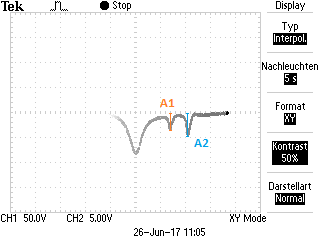
\includegraphics[width=0.7\textwidth]{TEK0002.png}
  \caption{Signal}
  \label{fig:signal}
\end{figure}
Dabei entspricht das Amplitudenverhältnis dem Isotopenverhältnis.
\begin{align}
  \frac{A_{\ce{^{87}Rb}} }{A_{\ce{^{85}Rb}} }=\frac{N_{\ce{^{87}Rb}} }{N_{\ce{^{85}Rb}} }  \label{eqn:verhalt}
\end{align}
Die Amplituden der Resonazen sind:
\begin{align*}
A_{\ce{^{87}Rb}}&=17&   & A_{\ce{^{85}Rb}}=26   \text{\,\,\, \footnote{Die Amplituden wurden mit Hilfe von dem Lineratool von Paint vermessen.}}.
\end{align*}
aus \eqref{eqn:verhalt} folgt für das Isotopenverhältnis
\begin{align*}
  \frac{N_{\ce{^{87}Rb}}}{N_{\ce{^{85}Rb}}}\approx 0,65 .
\end{align*}



\subsection{Quadratischer Zeemaneffekt}
Indem das größte gemessene Magnetfelde bei der Höchste Frequenz in den Zusatzterm der
durch den Quadratischen Zeemaneffekt entsteht aus der Formel \eqref{eqn:quadrat} einsetzt,
kann der quadratische Zeemaneffekt bei der Messung  abgeschätzt werden.
Für $\ce{^{87}Rb}$ beträgt die Hyperfeinstrukturaufspaltung
\begin{align*}
  \Delta E=\SI{4,53e-24}{\joule}
\intertext{und für $\ce{^{85}Rb}$}
  \Delta E=\SI{2,01e-24}{\joule}.
\end{align*}
...
